\section{Background}
\label{sec:-back}
\subsection{Problem Structure}
The forest coverage classification problem clearly fits into the 
category of a multiclass classification problem, in which we describe 
a classifier that maps from a feature vector to one of a series of 
possible output labels. The output labels are given below:

\begin{enumerate}
\item Spruce/Fir
\item Lodgepole Pine
\item Ponderosa Pine
\item Cottonwood/Willow
\item Aspen
\item Douglas-fir
\item Krummholz
\end{enumerate}

Unlike a binary classifier,  a multiclass classifier can quite easily 
reach error rates in excess of 50\%.  As we are dealing with data 
collected from a natural source, we 
expect to encounter a fair amount of noise within the data set.  We keep 
this in mind when selecting the classifiers enumerated in the following 
subsection, and when tuning hyperparameters which govern noise 
tolerance.

The feature vector provided for forest cover type classification is 
outlined in table \ref{table:featurelist}.  It contains a mix of 
continuous and discrete binary values.

The continuous features are graphed in figure \ref{fig:continuous_features},
and include elevation, slope and aspect, as well as distances to important
geographic points, such as water and roads. Examining these graphs, we 
conjecture that elevation may be one of the more important features: it 
looks like some cover types are almost entirely constrained to a 
small range of elevation.  While the other continuous features may be 
helpful later on, their importance is not immediately visible from a 
simple graph.

The discrete features, as visualized in figures \ref{fig:soil} 
and \ref{fig:wilderness}, account for multiclass features encoded with 
the one-hot encoding method. It is clear from these graphs that some 
cover types are more prevalent in certain wilderness areas or certain 
soil types. However, determining the forest cover by wilderness area 
or soil type alone proves impossible, as no wilderness area or soil 
type is the sole domain of any type of forest cover.  Therefore, we must 
integrate the discrete features into our model alongside the continuous 
features in order to produce an effective algorithm.

\begin{figure*}
\centering
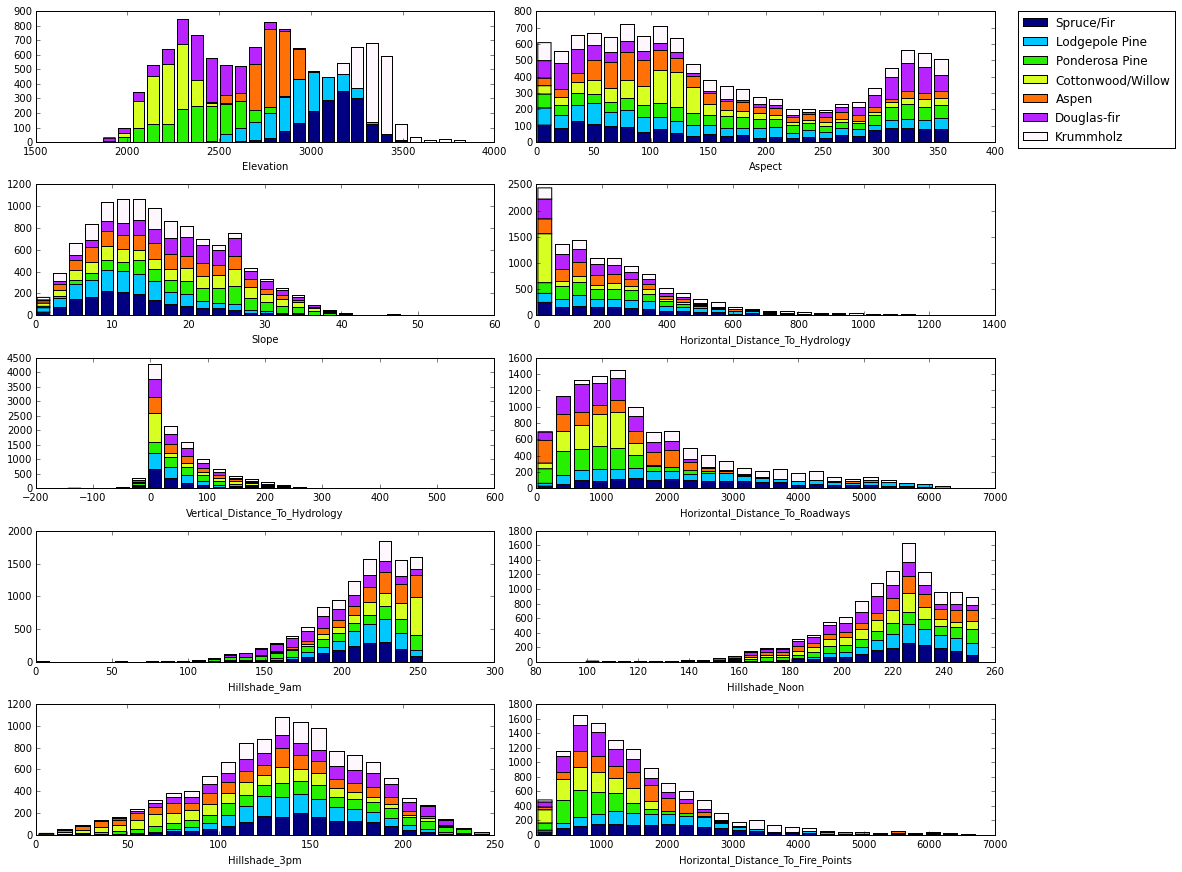
\includegraphics[width=\linewidth]{continuous}
 \caption{Histogram for continuous variables showing cover type distribution}
 \label{fig:continuous_features}
\end{figure*}

\begin{figure*}
\centering
\begin{minipage}{.5\textwidth}
  \centering
  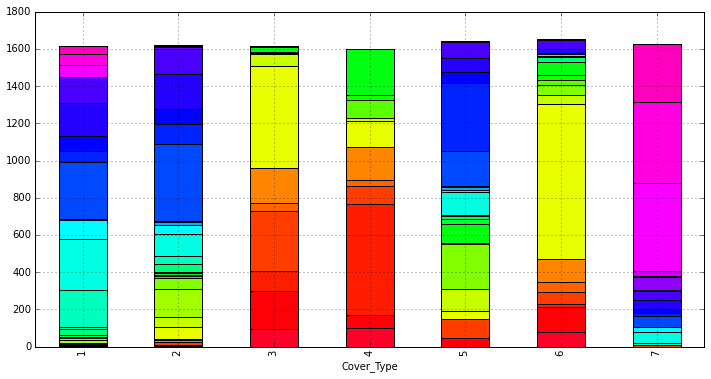
\includegraphics[scale=0.29]{soil_type}
  \captionof{figure}{prevalence of soil type aggregated by cover type}
  \label{fig:soil}
\end{minipage}%
\begin{minipage}{.5\textwidth}
  \centering
  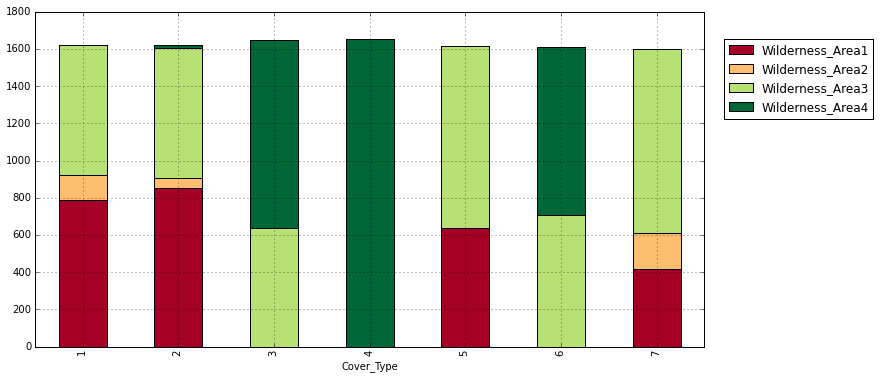
\includegraphics[scale=0.29]{wilderness}
  \captionof{figure}{Wilderness areas grouped by cover type}
  \label{fig:wilderness}
\end{minipage}
\end{figure*}

%\begin{figure*}
%\centering
%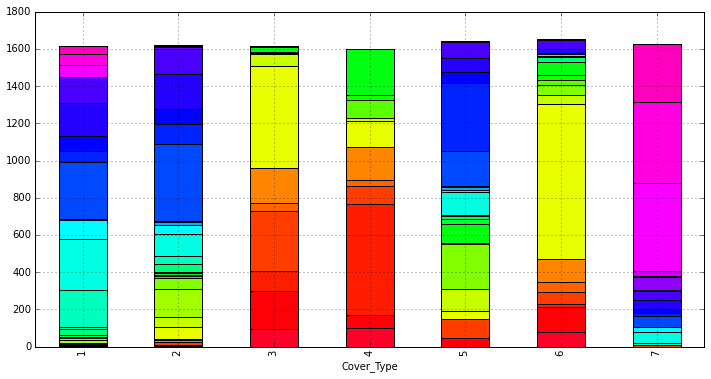
\includegraphics[scale=0.4]{soil_type}
% \caption{Soil types and accompanying cover types}
% \label{fig:soil}
%\end{figure*}

%\begin{figure*}
%\centering
%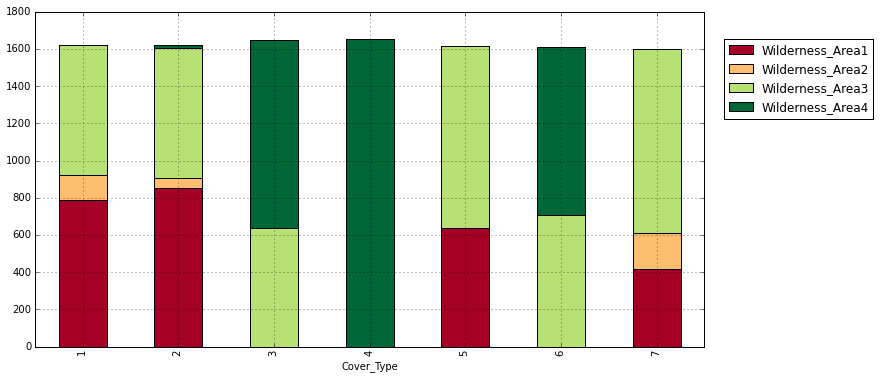
\includegraphics[scale=0.4]{wilderness}
% \caption{Wilderness types and accompanying cover types}
% \label{fig:wilderness}
%\end{figure*}

\subsection{Solution structure}
The classification solution we assemble to solve this problem involves 
a number of different machine learning models.  We began the project by 
attempting a Random Forest classifier, but eventually expanded to also 
make use of a Gradient Boost Machine, a Support Vector Machine, and a 
k-Nearest Neighbor classifier.  Each of these machines has its own 
strengths and weaknesses, which we will discuss as follows.  Each model 
has a number of hyperparameters that must be tuned properly before 
evaluating the total efficacy of such a technique: we will cover the 
tuning process in the following sections.

A Random Forest classifier\cite{breiman2001random} is an example of an 
ensemble method, a sort of mashup of decision trees with a machine 
learning technique called bootstrap aggregating, or, more colloquially, 
bagging\cite{bagging}.  Instead of constructing a single tree on the 
entirety of the training set, Random Forest constructs many smaller 
trees on randomly selected subsets of the training data.  This has a 
number of perks: Random Forests are resistant to artifacts of training 
set ordering and are highly robust in the face of noise and superfluous 
features.  Perhaps most importantly, Random Forests, by effectively 
averaging together a number of decision trees, can effectively mitigate 
the tendency of decision trees to overfit the training data.  As a 
small bonus, the structure of the algorithm allows for efficient 
parallelism, making this a very quick algorithm on a computer with 
sufficient cores.

When we began exploring the idea of adding further classifiers, we 
settled on the Grading Boosting Machine\cite{gbm} after some small 
amount of testing.  Like Random Forest, GBM is an ensemble method that 
constructs a number of subsidiary decision trees.  In this case, the 
algorithm combines decision trees with the idea of 
boosting\cite{boosting}.  Boosting is, in abstract, the process of 
combining a number of poor predictors into a single good predictor.  
In the case of a tree-based GBM, our process is superficially similar 
to bagging, insofar as we create trees based on repeatedly selecting 
subsets from the total training set.  The difference lies primarily in 
how we weight such trees.  Instead of relying largely on the sheer mass 
of trees, we instead attempt to select subtrees that will improve 
currently weak areas of the aggregate predictor.

k-Nearest Neighbor\cite{nearest} is arguably the simplest algorithm we 
deploy in the course of this paper.  We consider an n-dimensional 
graph (for a total of n features) over the feature space.  By populating 
the graph with our training examples, our predictor takes the form of 
simply checking the class of the k training examples that are closest 
to the testing instance.  This distance metric can be a simple 
Euclidean distance calculation, or one of a number of more complex 
metrics suited for particular problem domains.

Support Vector Machines\cite{support} share some commonalities with 
the k-NN algorithm as described above.  We repeat the process of 
populating an n-dimensional graph with training examples, and from 
there the algorithms diverge significantly.  k-NN is a lazy algorithm: 
that is to say, computation is generally delayed until it must actually 
compute the classification.  By contrast, an SVM is a non-lazy binary 
linear classifier.  The SVM attempts to generate a hyperplane that 
separates the graph into two distinct sets.  By utilizing the approach 
of one-hot encoding, we can cause SVM to carry out multiclass 
classification.  Our SVM model can be made resistant to overfitting, 
and SVMs in general can make use of the kernel trick to classify 
nonlinear functions.  In this case, we make use of the RBF\cite{rbf} 
kernel, which tends to be useful in smoothing out noisy data sets. 

Most of the algorithms we made use of for this classification problem 
were provided by scikit-learn, with a couple of important exceptions.  
When mixing our classifiers together into a voting body, we rolled our 
own method of voting.  In addition, the confusion matrix as detailed in 
figure \ref{fig:confusion} motivated a second layer of Random Forest 
classifier, where certain classes of classifications cause our system to 
double-check its work.  


%%% Local Variables: 
%%% mode: latex
%%% TeX-master: "main"
%%% End: 
